\documentclass{article}%
\usepackage[T1]{fontenc}%
\usepackage[utf8]{inputenc}%
\usepackage{lmodern}%
\usepackage{textcomp}%
\usepackage{lastpage}%
\usepackage{authblk}%
\usepackage{graphicx}%
%
\title{High cellular organization of pyoverdine biosynthesis in Pseudomonas aeruginosa: clustering of PvdA at the old cell poleemi\_274}%
\author{Danielle Robinson}%
\affil{State Key Laboratory for Agrobiotechnology and Key Laboratory of Crop Heterosis and Utilization (MOE), Beijing Key Laboratory of Crop Genetic Improvement, China Agricultural University, Beijing, China, \newline%
    National Plant Gene Research Centre (Beijing), Beijing, China}%
\date{01{-}01{-}2012}%
%
\begin{document}%
\normalsize%
\maketitle%
\section{Abstract}%
\label{sec:Abstract}%
On New Year's Day a severe outbreak of infections of ear bacteria, haemolytic anemia and arthritis prompted the San Diego County Department of Public Health to issue a warning asking everyone to take precautions against microorganisms during the colder months.\newline%
Two man were in critical condition, another had weakened bones and signs of a heart attack.\newline%
Friday, Dr. Hal Stup of VA Medical Center asked that you continue to take precautions, saying it is important that you use appropriate precautions when caring for others. Dr. Stup asked that people wash their hands after touching the wounds of their sick loved ones.\newline%
A link to all of Dr. Stup's pages can be found at his office.\newline%
"We never expected the way it turned out," Dr. Stup said. "We had no idea that the Escherichia{-}o{-}spans, not every strain, but the ones that have some risk of causing adverse health reactions, will be as severe as it is right now."\newline%
Dr. Stup said cases in recent years of people infected by a strain of Escherichia aegypti bacterium known as West Nile has been traced to people in the San Diego area.\newline%
To see Dr. Stup's timeline, click here.\newline%
To see Dr. Stup's timelines for other cold{-}related cases and medical conditions, click here.

%
\subsection{Image Analysis}%
\label{subsec:ImageAnalysis}%


\begin{figure}[h!]%
\centering%
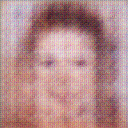
\includegraphics[width=150px]{500_fake_images/samples_5_160.png}%
\caption{A Man In A Suit And Tie Is Holding A Teddy Bear}%
\end{figure}

%
\end{document}